\documentclass{article}
%documentclass[draft]{article}


\usepackage[italian]{babel}
\usepackage[utf8]{inputenc}


\usepackage{graphicx} % Immagini fantastiche e...
\graphicspath{        % dove trovarle
  {./images/},
  %{../images/}        % Necessario se cartella chapters
}

%% Bibliografia
\usepackage{csquotes}
\usepackage{biblatex}
\addbibresource{bibl.bib}



% Per blocchi di codice
\usepackage{listings}

% Grafici direttamente in latex
\usepackage{tikz}
\usetikzlibrary{shapes,positioning,calc}
\colorlet{lightgray}{gray!20}

\usepackage{rotating} % per tabella ruotata
\usepackage{makecell}
%\usepackage[showframe=true]{geometry}
\usepackage{changepage}

% Immagini galleggiano
\usepackage{float}

\usepackage{color}

\usepackage{caption}
% per caption ad immagini in tab annidiate
\usepackage{subcaption}

\usepackage{hyperref} % lasciare per ultimo
%\hypersetup{colorlinks=true, linkcolor=blue, citecolor=black, plainpages=false, urlcolor=blue}
\hypersetup{colorlinks=true, linkcolor=black, citecolor=black, plainpages=false, urlcolor=blue}

% Usato nella copertina
\usepackage{wallpaper}


% Esempio di impostazione per listings
%\lstset{
%   language=Octave,
%   % language=Matlab,
%   showspaces=false,
%   showstringspaces=false,
%   basicstyle=\ttfamily,
%   %numbers=left,
%   numbers=none,
%   numberstyle=\small,
%   mathescape,
%}
%\newcommand*\lstinputpath[1]{\lstset{inputpath=#1}}
%\lstset{ % per apici e pedici nel codice
%  mathescape,
%  numbers=none
%}
%\lstset{ numbers=none }

% Simboli matematici
%\usepackage{amsthm}
%\usepackage{amsmath}
%\usepackage{amsfonts}
%\usepackage{mathabx} % per \topdoteq
%\usepackage{mathtools, amsthm}


% Comodo per evidenziare zone da modificare
\usepackage{todonotes} 

% Lorem ipsum...
\usepackage{lipsum} 


 
% ================================ %
%          Cose Personali          %
% ================================ %

% Alcune comodita' logico/matematiche
\let\ep\epsilon
\let\b\bullet
\let\iff\Leftrightarrow
\newcommand{\viff}{\Updownarrow}
\let\impl\Rightarrow

\newcommand{\norm}[1]{\lvert\lvert #1 \lvert\lvert}
\newcommand{\Norm}[1]{\Big\lvert \Big\lvert #1 \Big\lvert \Big\lvert}

\newcommand\N{\ensuremath{\mathbb{N}}}
\newcommand\R{\ensuremath{\mathbb{R}}}
\newcommand\Z{\ensuremath{\mathbb{Z}}}
\renewcommand\O{\ensuremath{\emptyset}}
\newcommand\Q{\ensuremath{\mathbb{Q}}}
\newcommand\C{\ensuremath{\mathbb{C}}}

% ================================ %
%            Il Documento          %
% ================================ %
\begin{document}

% ================================ %
%        Creo Prima Pagina         %
% ================================ %

\ThisCenterWallPaper{0.95}{polloPallido}
% Intestazione
% TODO Migliorare esteticamente
\begin{titlepage}
 	\centering
  \Huge{\textbf{Approfondimento di Intelligenza Artificiale}}\\
 	[30mm]
 	\centering
  \Huge{\textbf{Studente: Tristano Munini}}\\
 	%[25mm]
  %\raggedright
  %\Large{\textbf{Corso:}}\\
  %\Large{\textbf{TODO}}\\
 	[125mm]
 	\centering
  \LARGE{\underline{\textbf{ANNO ACCADEMICO 2019-2020}}}\\
\end{titlepage}

%% ================================ %
%%              Indice              %
%% ================================ %
%\tableofcontents
%\thispagestyle{empty}
%\cleardoublepage
%\setcounter{page}{1}


% ================================ %
%      Qua Inizia La Tesina        %
% ================================ %
%\abstract{
%  \lipsum[1]
%}

%\pagenumbering{gobble} % TODO REMOVE

%\input{./chapters/x.tex}
%!TEX TS-program = pdflatex
%!TEX root = main.tex
%!TEX encoding = UTF-8 Unicode

\section{Introduzione}

Questo approfondimento ha come oggetto le tecniche di \emph{Machine Learning} (ML) \emph{Generative Adversarial Network} (GAN) e \emph{Reinforcement Learning} (RL).
In  particolare nelle  prima sezione si  esplorano le tecniche generative, definendo prima i \emph{Variational  Autoencoder} e  poi le GAN.
Nella seconda sezione si definiscono i concetti alla base  del  \emph{Reinforcement Learning} e come le tecniche di ML possono essere sfruttate in questo ambito.
La terza  sezione illustra come si può combinare l'architettura GAN con tecniche prese dal mondo del RL per generare testi sintetici che siano verosimili.
Nello specifico si analizzano l'architettura SeqGAN \cite{SeqGAN} e la sua evoluzione LeakGAN \cite{LeakGAN}.
L'ultima sezione illustra brevemente un'implementazione delle LeakGAN scritta dagli stessi autori dell'articolo che la introduce \cite{LeakGAN}.

%!TEX TS-program = pdflatex
%!TEX root = main.tex
%!TEX encoding = UTF-8 Unicode


\section{GAN}
Uno tra i primi metodi che permettevano di generare immagini sintetiche faceva uso di una particolare versione di \emph{Auto-Encoder} i \emph{Variational Auto-Encoder}.
Come nel caso degli AE classici, i VAE hanno una struttura che ricorda una clessidra: la prima metà della rete permette di comprimere l'input, mappandolo in quello che viene chiamato spazio latente, di minor dimensione rispetto allo spazio di partenza;  la seconda metà, invece, prende l'input compresso e lo mappa nello spazio di partenza.
Durante il training si vuole ottimizzare la compressione in modo che non ci sia perdita di informazione, questo viene effettuato andando a minimizzare la distanza tra input originale ed input ricostruito.
Nei VAE, in corrispondenza del punto della rete in cui si raggiunge il livello massimo di compressione (\emph{bottleneck}), invece di essere generato il vettore compresso $z$, viene prodotta una coppia di vettori $\sigma$ e $\mu$ che descrivono una distribuzione di probabilità dei vettori compressi.
In questo modo è possibile campionare $z$ dalla distribuzione appena prima della decompressione.
Il campionamento non è un'operazione differenziabile e questo rende inapplicabile l'algoritmo della $backpropagation$, quindi risulta necessario effettuare quello che viene chiamato \emph{reparametrization trick}.
Rappresentando $z$ come $z = \mu + \sigma \odot \varepsilon$ in cui $\varepsilon \sim \mathcal{N}(0,1)$, quindi $\varepsilon$ è campionata da una distribuzione normale, è possible effettuare l'operazione di \emph{sampling} all'esterno della rete.
In questo modo $\mu$ e $\sigma$ possono essere utilizzati per il calcolo del gradiente e quindi usati durante la \emph{backpropagation}.

Dopo questa breve panoramica sulle VAE, ispirata alla lezione del MIT \cite{MIT_GEN}, ci si accorge che sono una soluzione astuta ma complessa e che le loro prestazioni sono vincolate strettamente allo spazio latente che si è trovato durante il training.
%TODO nota sul Disentanglement delle variabili che permette di avere controllo sulle singole caratteristiche delle immagini generate

Le \emph{Generative Adversarial Network} (GAN) sono state modellate appositamente per trovare un'altra soluzione al problema della creazione di immagini sintetiche.
Nelle GAN sono presenti due modelli che, citando \cite{GANTF}, \emph{``vengono addestrati simultaneamente da un processo contraddittorio. Un generatore ("l'artista") impara a creare immagini che sembrano reali, mentre un discriminatore ("il critico d'arte") impara a distinguere le immagini reali dai falsi''}.
Riformulando la frase si può dire che una GAN, come si vede in \autoref{fig:gan}, è composta da due reti: la prima viene chiamata Generatore $G$ ed il suo scopo è fornire in output un $x_{fake}$ che sembri appartenere alla distribuzione del \emph{dataset} reale fornito; la seconda, detta Discriminatore $D$, prende in input un $x_{fake}$ ed un $x_{real}$ estratto dal \emph{dataset} e deve riuscire a distinguere il dato reale da quello sintetico.
Quindi il training viene svolto in quattro momenti:
\begin{itemize}
  \item all'inizio $G$ a partire da del rumore randomizzo genera, basandosi sulle sue conoscenze attuali, un $x_{fake}$;
  \item successivamente $D$ stabilisce quale tra $x_fake$ ed un $x_real$ fornito è sintetico;
  \item la prestazione di $D$ viene valutata con il \emph{ground truth} e con questa può essere effettuata la \emph{backpropagation} su $D$;
  \item con l'output del discriminatore è possibile determinare anche la prestazione di $G$, infatti se questo è riuscito a confondere $D$ significa che sta raggiungendo una buona conoscenza del dominio.
\end{itemize}
Notare come $G$ sia in grado di mappare del rumore casuale nello spazio delle \emph{feature} del dominio e che quindi, una volta allenato, possa essere sfruttato molto facilmente: basterà avere del rumore da cui partire.
Si può quindi dire che $G$ opera come il decoder di un AE con un particolare spazio latente molto semplice.
\begin{figure}[ht]
  \centering
  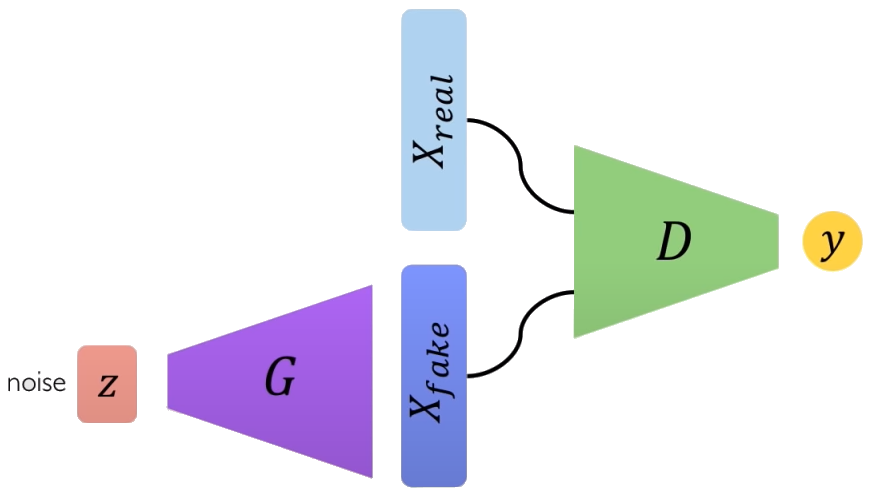
\includegraphics[width=.7\textwidth]{GAN/arch.png}
  \caption{Architettura di una generica GAN (dalle slide in \cite{MIT_GEN})}
  \label{fig:gan}
\end{figure}
Rispetto ai $VAE$ le $GAN$ risultano non solo più intuitive ma permettono anche di raggiungere prestazioni veramente sorprendenti, come si può vedere in \cite{GAN_HD}, in cui anche gli esperti umani vengono ingannati dai prodotti della rete.

Va fatto notare però che le GAN sono notoriamente difficili da allenare %\cite{HARD_GAN}
\todo{leggere xke GAN difficili}
, basti pensare che prima dell'allenamento entrambe le sotto-reti non hanno alcuna conoscenza del dominio e si chiede loro di guidarsi a vicenda.
Se il discriminatore converge rapidamente è possibile che dia una valutazione così bassa al generatore da causare il \emph{vanishing gradient problem}, rendendo quindi impossibile che $G$ possa migliorarsi.
Un altro problema noto è quello del \emph{model collapse} che si verifica quando $G$ riproduce molto bene soltanto una piccola frazione del dominio.
In questo modo riesce ad ottenere punteggi molto alti ma a discapito della generalità.


% L'efficacia di questa tecnica e' lampante quando si parla di immagini...
%In questo caso si fa riferimento alla possibilità di utilizzare le GAN come generatori di immagini sintetiche indistinguibili da quelle reali, in \cite{GAN_HD} si può osservare il livello di dettaglio impressionante che queste reti sono in grado di produrre.


\todo[inline]{aggiungere robe dal paper originale se si deve allungare}

$$
min_G max_D V(D,G) = \E_{x \sim P_real(x)} [ log D(x) ] 
+
\E_{z \sim P_z(x)} [ log ( 1 - D(G(x)) ]
$$ 
\todo{inserire formula per chiarire training e obj}

\clearpage


%% ================================ %
%%           Bibliografia           %
%% ================================ %
\cleardoublepage
\printbibliography



\end{document}
